\documentclass[a4paper, 12pt]{article}
\usepackage[total={17cm,25cm}, top=2.5cm, left=2.5cm, right=2.5cm,  includefoot]{geometry}
\usepackage[utf8]{inputenc}
\usepackage{array}
\usepackage{multirow}
\usepackage{hhline}
\usepackage{gensymb}
\usepackage{graphicx}
\graphicspath{ {} }
\usepackage[czech]{babel}
\usepackage{enumitem}
\usepackage{pdfpages}
\usepackage{amsmath}
\usepackage{verbatim}
\usepackage{listings}
\usepackage{hyperref}
\usepackage{amssymb}


\pagestyle{empty} % vypne číslování stránek




\usepackage[OT2,OT1]{fontenc}
\newcommand\cyr
{
\renewcommand\rmdefault{wncyr}
\renewcommand\sfdefault{wncyss}
\renewcommand\encodingdefault{OT2}
\normalfont
\selectfont
}
\DeclareTextFontCommand{\textcyr}{\cyr}
\def\cprime{\char"7E }
\def\cdprime{\char"7F }
\def\eoborotnoye{\char’013}
\def\Eoborotnoye{\char’003}
\setlength{\parindent}{1em} 
%\setlength{\parskip}{0.5ex}


\begin{document}

\begin{titlepage}
\begin{center}
\Huge
\vspace*{4.5cm}
Algoritmy v digitální kartografii \\
\vspace{0.2cm}

\Large  
Geometrické vyhledávání bodu\\
\vspace{0.2cm}

\normalsize  
Zimní semestr 2018/2019\\
(oprava: 5. 11. 2018)
\vspace{14cm}
\end{center}

\begin{flushright}
\Large
Tereza Kulovaná \\
Markéta Pecenová \\
\end{flushright}

\end{titlepage}


\pagestyle{plain}     % zapne obyčejné číslování
\setcounter{page}{1}  % nastaví čítač stránek znovu od jedné

\tableofcontents
\newpage

\section{Zadání}
Zadání úlohy bylo staženo ze stránek předmětu \href{https://web.natur.cuni.cz/~bayertom/index.php/teaching/algoritmy-v-digitalni-kartografii}{155ADKG}.

\begin{figure}[h!]
	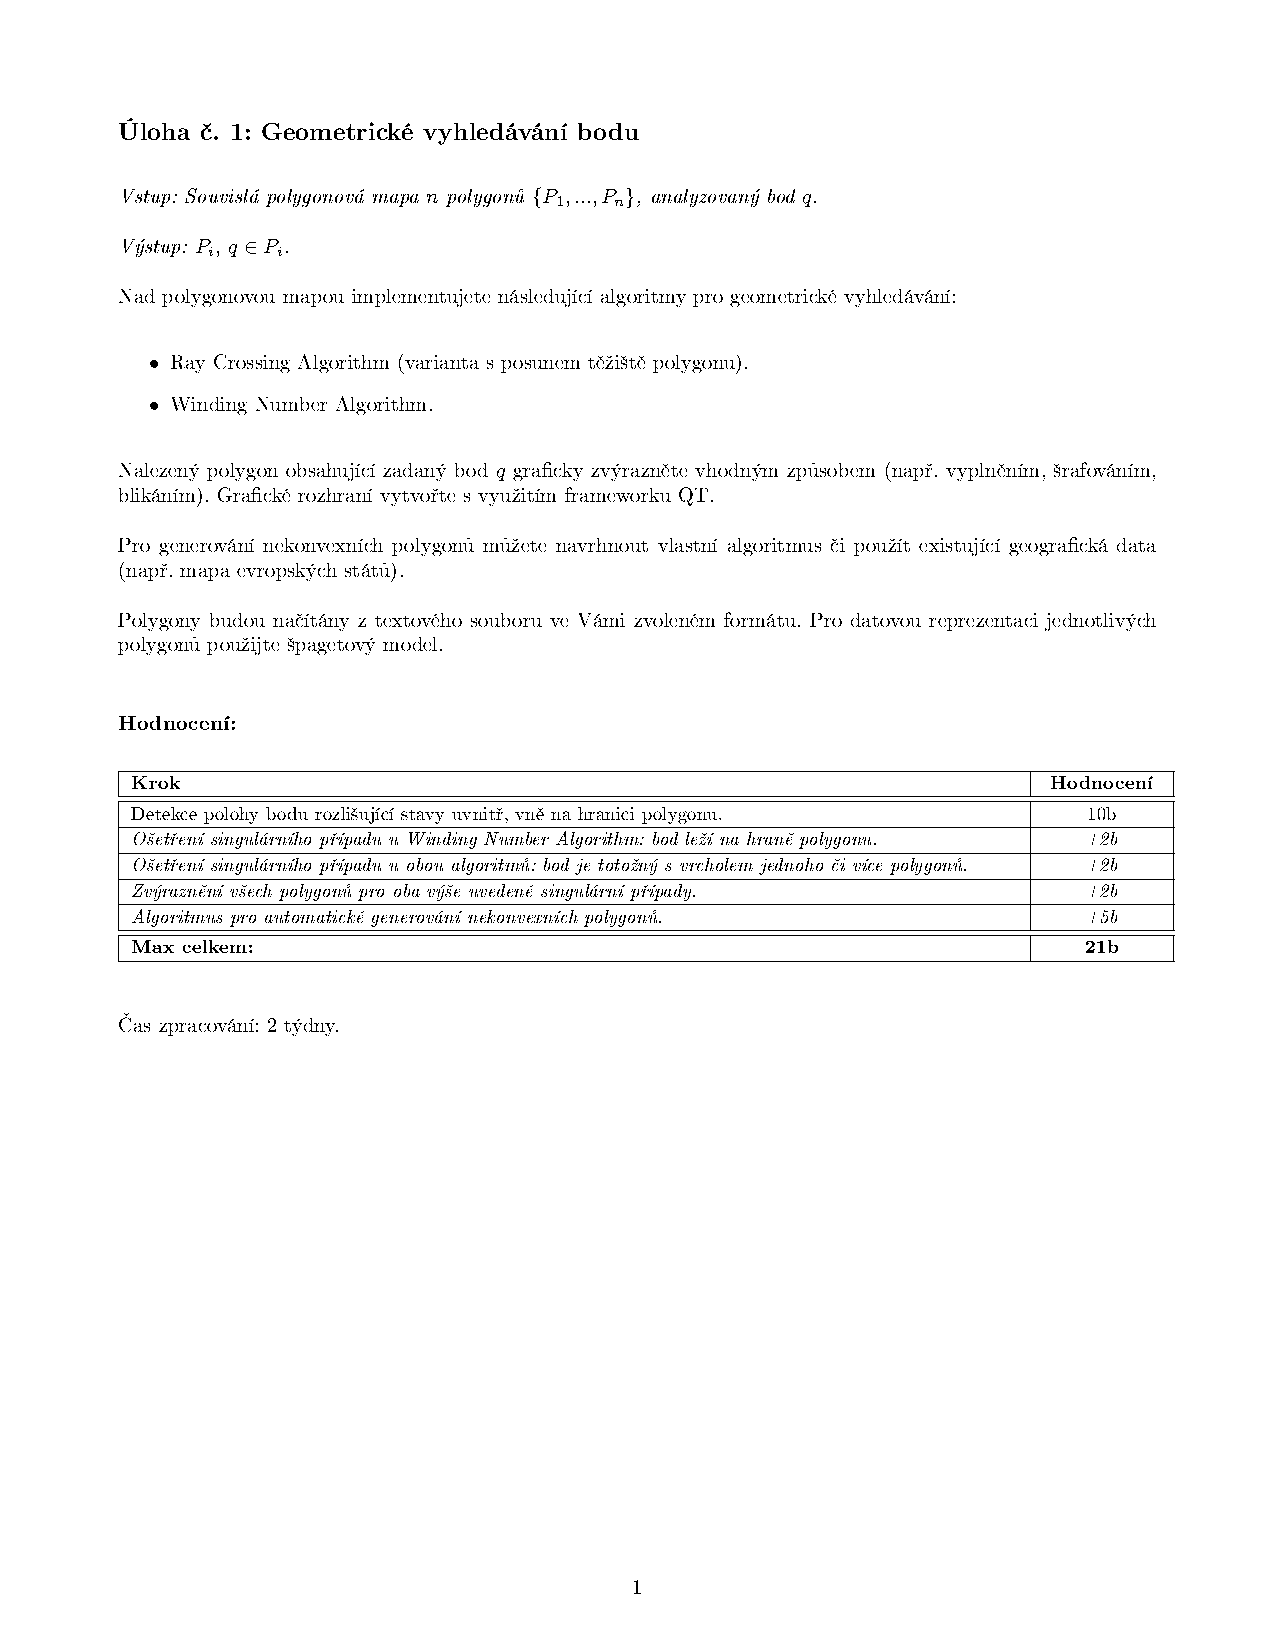
\includegraphics[clip, trim=0cm 10cm 0cm 3cm, width=1.0\textwidth]{./pictures/zadani.pdf}
\end{figure}

V rámci této úlohy byly implementovány bonusové úlohy č. 1-3. Poslední bonusovou úlohu, generování nekonvexních polygonů, tato aplikace neposkytuje.
\clearpage

\section{Popis a rozbor problému}
Úloha \textit{Geometrické vyhledávání bodu} se zabývá vytvořením aplikace, která umožní uživateli zjistit polohu jím zvoleného bodu $q$ vzhledem k příslušnému mnohoúhelníku. Jako vhodné řešení bylo vzhledem k náročnosti problému zvoleno opakované určovnání polohy bodu $q$ a mnohoúhelníku.

Existují dva základní druhy mnohoúhelníků (pro účely této úlohy je nazývejme polygony), konvexní a nekonvexní. Konvexní polygon je takový polygon, jehož všechny diagonály leží uvnitř polygonu a žádná z nich neprotíná jeho hranu. Konkávní polygon tuto podmínku nesplňuje. Pro představu je níže přiložen obrázek obou druhů polygonů.

\begin{figure}[h!]
	\centering
	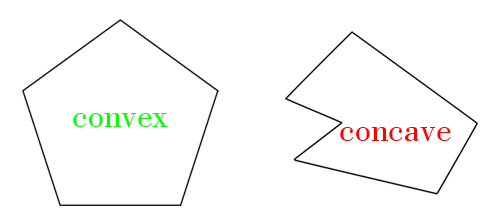
\includegraphics[width=13cm]{./pictures/convex_concave.png}
	\caption{Ukázka konvexního (vlevo) a konkávního polygonu (vpravo) (\href{https://www.nextgurukul.in/nganswers/ask-question/answer/What-is-concave-38-convex-polygon-/Understanding-Quadrilaterals/75323.htm}{\textsl{zdroj}})}
\end{figure}

Z výše uvedeného vyplývá, že bod $q$ může vůči polygonu $P$ zaujímat 4 pozice:
\begin{enumerate}
\item Bod $q$ se nalézá uvnitř polygonu $P$.
\item Bod $q$ se nalézá vně polygonu $P$.
\item Bod $q$ se nalézá na hraně polygonu $P$.
\item Bod $q$ se nalézá ve vrcholu polygonu $P$.
\end{enumerate}

Pro účely této aplikace byly zvoleny výpočetní algoritmy \textit{Ray Crossing} a \textit{Winding Number}, jejichž princip je vysvětlen v následující kapitole.

\section{Algoritmy}
Tato kapitola se zabývá popisem algoritmů, které byly v aplikaci implementovány. 

\subsection{Ray Crossing Algorithm}
Prvním zvoleným algoritmem je tzv. \textit{Ray Crossing Algorithm} neboli \textit{Paprskový algoritmus}. Svůj název získal po způsobu, jakým řeší nalezení polohy bodu vůči polygonu. Tento algoritmus je primárně využíván pro konvexní polygony, lze ho však zobecnit a využít ho i pro nekonvexní polygony. 

Mějme polygon $P$ a daný bod $q$. Z bodu $q$ veďme libovolný počet polopřímek (paprsků). Princip algoritmu je založen na vyhodnocení počtu průsečíků $k$, které vzniknou protnutím paprsků vedených z bodu $q$ s hranami polygonu $P$. Pro $k$ mohou nastat dvě situace:
\begin{enumerate}
\item Hodnota $k$ je rovna lichému číslu $\rightarrow$ bod $q$ se nachází uvnitř polygonu $P$.
\item Hodnota $k$ je rovna sudému číslu $\rightarrow$ bod $q$ se nachází vně polygonu $P$.
\end{enumerate}

Základní varianta algoritmu neošetřuje problémové situace, které mohou během výpočtu nastat. Konkrétně se jedná o dvě níže uvedené situace:

\begin{enumerate}
\item $q == p_i$
\item $q$ leží na polygonové hraně tvořené vrcholy $p_i$ a $p_{i+1}$
\end{enumerate}

Pro eliminaci těchto tzv. singularit je vhodné použít modifikovanou variantu algoritmu, která redukuje souřadnice bodů polygonu k bodu $q$ (viz krok 2(I.) níže). 

Zjednodušený zápis takto modifikovaného algoritmu lze zapsat způsobem uvedeným níže:
\begin{enumerate}
\item Načtení bodů polygonu $p_i$, počet průsečíků $k$ = 0
\item Postupně pro všechny $p_i$ opakuj kroky I–IV:
\begin{enumerate}[label=\Roman*.]
\item 	Redukce souřadnic bodu $p_i$ k bodu $q$:\\
$x'_i = x_i - x_q$\\
$y'_i = y_i - y_q$
\item 	Podmínka $(y'_i > 0)\&\&(y'_{i-1} \leq 0)\|(y'_{i-1} > 0)\&\&(y'_{i} \leq 0)$
\item 	Je-li podmínka splněna: $x'_m = \frac{x'_i y'_{i-1} - x'_{i-1} y'_i}{y'_i - y'_{i-1}}$
\item Podmínka $(x'_m > 0) \rightarrow k = k + 1$ 
\end{enumerate}
\item Výpočet $k\%2$
\item Vyhodnocení $k$ (liché $k \rightarrow q$ náleží $P$; sudé $k \rightarrow q$ nenáleží $P$)
\end{enumerate}

\subsection{Winding Number Algorithm}
Druhý algoritmus použitý v aplikaci je tzv. \textit{Winding Number Algorithm} neboli \textit{Metoda ovíjení}, který je vhodný pro nekonvexní polygony. Princip tohoto algoritmu je založen na součtovém úhlu $\omega$.

Mějme polygon $P$ a bod $q$, na kterém stojí pozorovatel. Nachází-li se $q$ uvnitř $P$, pak pozorovatel, který by si přál postupně vidět všechny vrcholy polygonu, se musí otočit celkem o $2\pi$. Výsledkem algoritmu je pak tzv. Winding number $\omega$, které říká, o kolik otáček se pozorovatel otočil: \\ \\
$\Omega = \frac{1}{2\pi} \sum_{i=1}^n \omega_i$\\ \\
Zde se hodí zdůraznit, že záleží na zvoleném směru otáčení. Otáčí-li se pozorovatel ve směru chodu hodinových ručiček, úhly se sčítají. V opačném směru se od sebe úhly odečítají a $\omega$ by vyšlo záporné. Během výpočtů je také nutno zavést určitou toleranci $\epsilon$, která pokrývá chyby způsobené zaokrouhlováním.
Z výše uvedených vztahů vyplývá:
\begin{enumerate} 
\item $w = 2\pi \rightarrow$ $q$ se nachází uvnitř $P$
\item  $w < 2\pi \rightarrow$ $q$ se nachází vně $P$
\end{enumerate}

Mezi singularity pro tento algoritmus patří pouze případ, je-li $q\approx p_i$. Tento problém byl vyřešen zavedením speciální třetí návratové hodnoty, která ošetřuje tento případ.\\

Zjednodušený zápis algoritmu:

\begin{enumerate}
\item Načtení bodů polygonu, úhel $\omega = 0$, tolerance $\epsilon = 1e-10$
\item Orientace $o_i$ bodu $q$ ke straně $p_i, p_{i+1}$
\item Postupně pro všechny orientované trojice $p_i, q, p_{i+1}$ opakuj kroky I-III:
\begin{enumerate}[label=\Roman*.]
\item Výpočet úhlu $\omega_i = \sphericalangle p_i, q, p_{i+1}$
\item Podmínka ($q$ je vlevo) $\rightarrow \omega = \omega + \omega_i$
\item Jinak $\omega = \omega - \omega_i$
\end{enumerate}
\item Podmínka $(\mid \omega - 2\pi \mid) < \epsilon \rightarrow q$ náleží $P$
\item Jinak  $q$ nenáleží $P$
\end{enumerate}

\section{Problematické situace}
V úloze bylo nutné ošetřit sigularity, zda bod $q$ neleží v hraně některého z polygonů či v jejich vrcholech. Pro vyřešení tohoto problému byla použita metoda \textsl{getDistanceEdgeQ} třídy \textbf{Algorithms}, která porovnává vzdálenost dvou bodů $p_1$ a $p_2$ na přímce $p$ se sumou vzdáleností těchto bodů k danému bod $q$. Je-li rozdíl vzdáleností menší než mezní hodnota $\epsilon$, je bod $q$ vyhodnocen, že leží na přímce.\\

$\mid d_{p_1,p_2} - \sum(d_{p_1,q} + d_{q,p_2}) \mid  < \epsilon \rightarrow q$ náleží přímce $p$.

\section{Vstupní data}
Aplikace požaduje dva druhy vstupních dat:

\begin{enumerate}
\item soubor daných polygonů
\item daný bod $q$
\end{enumerate}

Seznam bodů jednotlivých polygonů je uložen v textovém souboru polygon.txt. Pro vykreslení jednotlivých polygonů v aplikaci je nutno tento soubor do aplikace nahrát pomocí tlačítka \textsl{Load}. K vygenerování souřadnic bodů byla použita online aplikace ze stránek mobilefish.com. Struktura souboru s polygony je následující:\\

\noindent
\textsl{První řádek}: počet polygonů v souboru\\
\textsl{Sloupec 1}: číslo polygonu, jehož součástí daný bod je\\
\textsl{Sloupec 2}: souřadnice X daného bodu polygonu\\
\textsl{Sloupec 3}: souřadnice Y daného bodu polygonu\\

Bod $q$ není součástí textového souboru, do aplikace vstupuje na základě ručního zadání uživatelem. Pro zadání bodu je nutné v aplikaci kliknout levým tlačítkem myši do okna s polygony.

\section{Výstupní data}
Výstupem úlohy je vypsání v grafickém okně aplikace, v jaké poloze se analyzovaný bod vůči polygonům nachází. Polygony, kterým bod náleží, jsou barevně zvýrazněny.

\section{Aplikace}
V následují kapitole je představen vizuální vzhled vytvořené aplikace tak, jak ji vidí prostý uživatel.

\begin{figure}[h!]
	\centering
	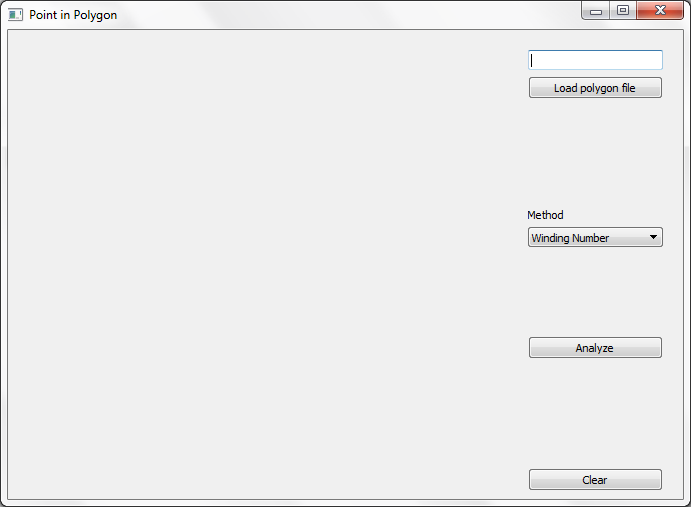
\includegraphics[width=10cm]{./pictures/gui_default.png}
	\caption{Aplikace ve výchozím stavu}
\end{figure}

\begin{figure}[h!]
	\centering
	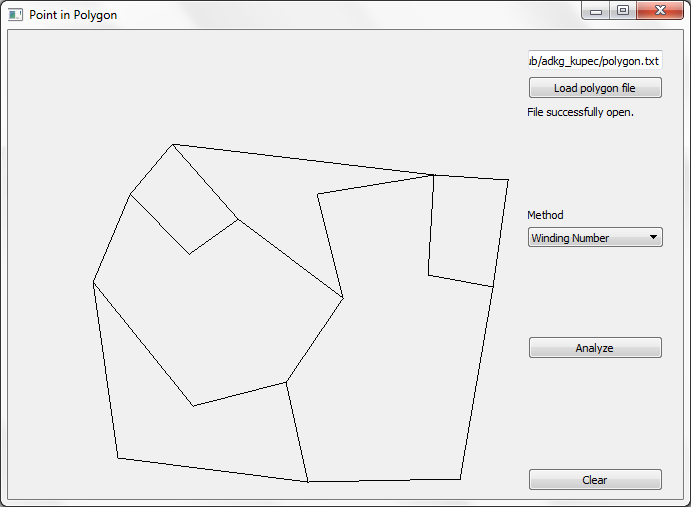
\includegraphics[width=10cm]{./pictures/gui_load.png}
	\caption{Aplikace po nahrání polygonů}
\end{figure}

\begin{figure}[h!]
	\centering
	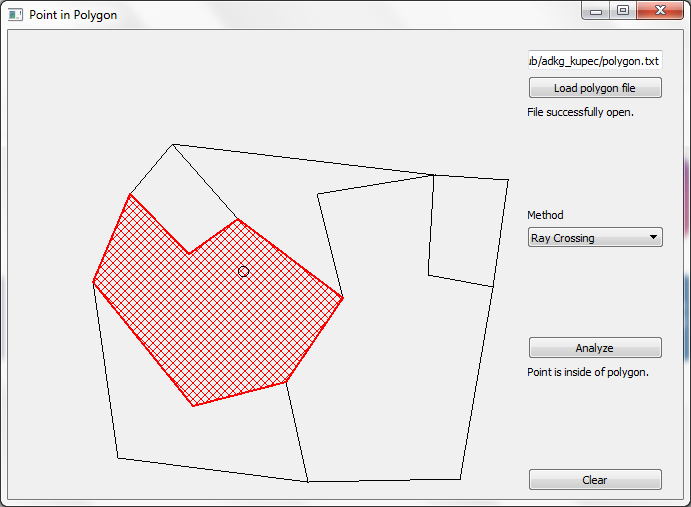
\includegraphics[width=11cm]{./pictures/gui_ray.png}
	\caption{Výstup při použití \textit{Ray Crossing Algorithm}}
\end{figure}

\begin{figure}[h!]
	\centering
	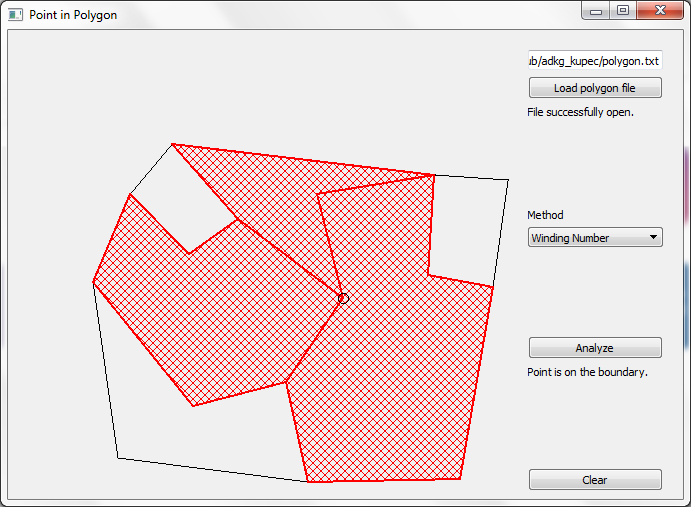
\includegraphics[width=11cm]{./pictures/gui_winding.png}
	\caption{Výstup při použití \textit{Winding Number Algorithm} pro $q$ ležící ve více vrcholech polygonů}
\end{figure}

\clearpage
 
\section{Dokumentace}
Tato kapitola obsahuje dokumentaci k jednotlivým třídám.

\subsection{Algorithms}
Třída \textsl{Algorithms} obsahuje metody, které určují polohu zvoleného bodu $q$ vzhledem k polygonu. Dále obsahuje pomocné metody pro výpočet úhlu mezi třemi body a na zjištění polohy bodu vzhledem k přímce. 

\subsubsection{getPositionRay}
Metoda \textbf{getPositionRay} určuje polohu bodu $q$ vzhledem k polygonu za použití algoritmu \textsl{Ray Crossing}. Na vstupu je bod třídy QPoint a vektor bodů polygonu. Návratová hodnota je typu \textsl{int}.

\textbf{Input}:
\begin{itemize}
\item $QPoint$ q
\item $std::vector\textless QPoint\textgreater$ pol
\end{itemize}

\textbf{Output}:
\begin{itemize}
\item 0 $\rightarrow$ bod se nachází vně polygonu
\item 1 $\rightarrow$ bod se nachází uvnitř nebo na hraně polygonu
\item -1 $\rightarrow$ bod se nachází na hraně polygonu
\end{itemize}

\subsubsection{getPositionWinding}
Metoda \textbf{getPositionWinding} určuje polohu bodu $q$ vzhledem k polygonu za použití algoritmu \textsl{Winding Number}. Na vstupu je bod třídy QPoint a vektor bodů polygonu. Návratová hodnota je typu \textsl{int}.

\textbf{Input}:
\begin{itemize}
\item $QPoint$ q
\item $std::vector\textless QPoint\textgreater$ pol
\end{itemize}

\textbf{Output}:
\begin{itemize}
\item 0 $\rightarrow$ bod se nachází vně polygonu
\item 1 $\rightarrow$ bod se nachází uvnitř polygonu
\item -1 $\rightarrow$ bod se nachází na hraně polygonu
\end{itemize}

\subsubsection{getPointLinePosition}
Metoda \textbf{getPointLinePosition} určuje polohu bodu $q$ vzhledem k přímce tvořené dvěma body. Na vstupu jsou souřadnice $x$ a $y$ pro 3 body typu \textit{double}, návratová hodnota je typu \textit{int} podle výsledku. 

\textbf{Input}:
\begin{itemize}
\item $double$ $x_q$
\item $double$ $y_q$
\item $double$ $x_1$
\item $double$ $y_1$
\item $double$ $x_2$
\item $double$ $y_2$
\end{itemize}

\textbf{Output}:
\begin{itemize}
\item 0 $\rightarrow$ bod se nachází vpravo od přímky
\item 1 $\rightarrow$ bod se nachází vlevo od přímky
\item -1 $\rightarrow$ bod se nachází na přímce
\end{itemize}

\subsubsection{getTwoVectorsAngle}
Metoda \textbf{getTwoVectorsAngle} počítá úhel mezi dvěma vektory. Na vstupu jsou souřadnice $x$ a $y$ pro 4 body typu \textit{double}, návratová hodnota typu \textit{double} vrací velikost úhlu v radiánech.

\textbf{Input}:
\begin{itemize}
\item $double$ $x_1$
\item $double$ $y_1$
\item $double$ $x_2$
\item $double$ $y_2$
\item $double$ $x_3$
\item $double$ $y_3$
\item $double$ $x_4$
\item $double$ $y_4$
\end{itemize}

\textbf{Output}:
\begin{itemize}
\item double 
\end{itemize}

\subsubsection{getDistanceEdgeQ}
Metoda \textbf{getDistanceEdgeQ} počítá, zda se bod nenachází na přímce na základě porovnání vzdálenosti mezi dvěma body na přímce se sumou vzdáleností těchto bodů k bodu $q$. Je-li rozdíl menší než zadané $\epsilon$, bod leží na přímce. Návratová hodnota je typu \textsl{int}.

\textbf{Input}:
\begin{itemize}
\item $double$ $x_1$
\item $double$ $y_1$
\item $double$ $x_2$
\item $double$ $y_2$	
\end{itemize}

\textbf{Output}:
\begin{itemize}
\item -1 $\rightarrow$ bod $q$ leží na přímce
\item 2 $\rightarrow$ bod $q$ neleží na přímce
\end{itemize}

\subsection{Draw}
Třída \textsl{Draw} obsahuje metody, které slouží k vykreslení polygonů, analyzovaného bodu $q$ a výstupních dat.

\subsubsection{paintEvent}
Metoda \textbf{paintEvent} vykresluje polygony a analyzovaný bod $q$. Návratová hodnota je typu \textsl{void}.

\textbf{Input}:
\begin{itemize}
\item QPaintEvent *e
\end{itemize}

\subsubsection{mousePressEvent}
Metoda \textbf{mousePressEvent} slouží k načtení souřadnic bodu $q$. Návratová hodnota je typu \textsl{void}.

\textbf{Input}:
\begin{itemize}
\item QMouseEvent *e
\end{itemize}

\subsubsection{clearCanvas}
Metoda \textbf{clearCanvas} slouží k vymazání všech vykreslených dat. Metoda neobsahuje žádné proměnné na vstupu a návratová hodnota je typu \textsl{void}.

\subsubsection{fillPolygon}
Metoda \textbf{fillPolygon} barevně vyšrafuje polygon, ve kterém se nachází analyzovaný bod $q$. Návratová hodnota je typu \textsl{void}.

\textbf{Input}:
\begin{itemize}
\item $std::vector\textless std::vector\textless QPoint\textgreater \textgreater$ poly\_fill
\end{itemize}

\subsubsection{loadPolygon}
Metoda \textbf{loadPolygon} slouží k nahrání bodů jednotlivých polygonů do aplikace.  Součástí metody je i kontrola, zda se soubor úspěšně nahrál, zda vůbec obsahuje nějaké polygony a zda jsou polygony tvořeny aspoň 3 body. Návratová hodnota je typu \textsl{QString} vrací hlášku, zda byly polygony úspěšně nahrány.

\textbf{Input}:
\begin{itemize}
\item const char* path
\end{itemize}

\textbf{Output}:
\begin{itemize}
\item QString
\end{itemize}

\subsection{Widget}
Metody třídy \textbf{Widget} slouží pro práci uživatele s aplikací. Až na jednu výjimku nemají metody na vstupu nic, návratové hodnoty všech metod jsou typu \textsl{void}.

\subsubsection{writeResult}
Metoda \textbf{writeResult} vrací polohu bodu $q$ vzhledem k polygonu na základě vstupní hodnoty typu \textit{int}.

\textbf{Input}:
\begin{itemize}
\item int
\end{itemize}

\subsubsection{on\_load\_button\_clicked}
Metoda \textbf{on\_load\_button\_clicked} načítá data z textového formátu. Uživatel sám vyhledává cestu k požadovanému souboru.

\subsubsection{on\_analyze\_button\_clicked}
Metoda \textbf{on\_analyze\_button\_clicked} vypisuje na obrazovku polohu bodu $q$ vzhledem k polygonům po zvolení požadovaného algoritmu a kliknutí na tlačítko \textsl{Analyze}.

\subsubsection{on\_clear\_button\_clicked}
Metoda \textbf{on\_clear\_button\_clicked} vrací aplikaci do výchozí polohy smazáním všeho, co bylo vykresleno. 

\clearpage
\section{Závěr}
V rámci úlohy \textit{Geometrické vyhledávání bodu} byla vytvořena aplikace, která určuje polohu analyzovaného bodu $q$ vzhledem k polygonu. Z důvodu větší časové náročnosti úlohy než obě autorky původně očekávaly nebyly implementovány všechny bonusové úlohy a některé části kódu mohly být řešeny lépe. Tato opravená verze technické zprávy je aktualizována o několik vzorců a o text v sekci Zadání. 

Jedná se například o použití tříd QPoint a QPolygon, které na vstupu mají hodnoty typu \textit{int} a které mohly být nahrazeny třídami QPointF a QPolygonF, jež na vstupu mají hodnot typu \textit{float}, což je pro práci se souřadnicemi bodů praktičtější. Dále jako ne zrovna nejšťastnější řešení hodnotíme množství vstupních hodnot, které mají na vstupu metody \textit{getPointLinePosition}, \textit{getTwoVectorsAngle} a \textit{getDistanceEdgeQ} třídy \textbf{Algorithms}. Vhodné by bylo nahradit jednotlivé souřadnice třídou QPoint, resp. QPointF. 

Dále mohlo být implementováno více kontrolních podmínek pro načítání bodů polygonu z textového souboru, například ošetření, zda soubor neobsahuje text, zda všechny body mají $x$ a $y$ souřadnici apod. Umisťování bodu $q$ do hran či vrcholů polygonů vyžaduje notnou dávku trpělivosti, aby se zobrazil korektní výsledek. Experimentálně bylo zjištěno, že aplikace zvládá lépe (tzn. je potřeba méně pokusů na kliknutí) zobrazovat polohu bodu $q$ ve vrcholech než v hranách, ač obě situace jsou v kódu ošetřené. 

Úloha přinesla i pozitivní přínos v tom směru, že se autorky mohly potrénovat v psaní kódu v jazyce C++ a oprášit své znalosti psaní v prostředí LaTeX.

\clearpage

\section{Zdroje}
\begin{enumerate}
\item  \textsl{BAYER, Tomáš. Geometrické vyhledávání bodů} [online][cit. 24. 10. 2018]. \\
Dostupné z: \href{https://web.natur.cuni.cz/~bayertom/images/courses/Adk/adk3.pdf}{https://web.natur.cuni.cz}
\item  \textsl{What is concave \& convex polygon?} [online][cit. 23. 10. 2018]. \\
Dostupné z: \href{https://www.nextgurukul.in/nganswers/ask-question/answer/What-is-concave-38-convex-polygon-/Understanding-Quadrilaterals/75323.htm}{https://www.nextgurukul.in}
\item \textsl{Record XY mouse coordinates} [online][cit. 23. 10. 2018].\\
Dostupné z: \href{https://mobilefish.com/services/record_mouse_coordinates/record_mouse_coordinates.php}{https://mobilefish.com/}\\

\end{enumerate}
\end{document}




%problematická situace na hrane a jeji ošetření winding
%osetřeno,aby polygony měli min 3 body
